% ============================================================
% Auxiliary boundary data and the failure of intrinsic coherence
% in a finite-nerve route for spectral causal theory
% ============================================================
\documentclass[11pt,a4paper]{article}

\usepackage[utf8]{inputenc}
\usepackage[T1]{fontenc}
\usepackage{amsmath,amssymb,amsthm}
\usepackage{mathtools}
\usepackage{enumitem}
\usepackage{booktabs}
\usepackage{tikz}
\usetikzlibrary{calc,arrows.meta,positioning,decorations.pathreplacing,backgrounds}
\usepackage[margin=2.5cm]{geometry}
\usepackage{hyperref}

\hypersetup{
  colorlinks=true,
  linkcolor=blue!60!black,
  citecolor=blue!60!black,
  urlcolor=blue!60!black,
  pdfauthor={David Alfyorov},
  pdftitle={Auxiliary boundary data and the failure of intrinsic coherence in a finite-nerve route for spectral causal theory},
  pdfsubject={Spectral Causal Theory, finite-nerve boundary operators}
}

%%% Theorem environments
\theoremstyle{plain}
\newtheorem{theorem}{Theorem}[section]
\newtheorem{proposition}[theorem]{Proposition}
\newtheorem{lemma}[theorem]{Lemma}
\newtheorem{corollary}[theorem]{Corollary}

\theoremstyle{definition}
\newtheorem{definition}[theorem]{Definition}
\newtheorem{example}[theorem]{Example}
\newtheorem{construction}[theorem]{Construction}

\theoremstyle{remark}
\newtheorem{remark}[theorem]{Remark}

%%% Custom commands
\newcommand{\NN}{\mathbb{N}}
\newcommand{\ZZ}{\mathbb{Z}}
\newcommand{\cU}{\mathcal{U}}
\newcommand{\cN}{\mathcal{N}}
\newcommand{\cT}{\mathcal{T}}
\newcommand{\swapAB}{\mathrm{swap}_{01}}
\newcommand{\swapAC}{\mathrm{swap}_{02}}
\newcommand{\swapBC}{\mathrm{swap}_{12}}
\newcommand{\chosenface}{\varphi}

\begin{document}

\title{Auxiliary boundary data and the failure of intrinsic coherence\\
  in a finite-nerve route for spectral causal theory}

\author{David Alfyorov\\[4pt]
  \small\textit{davidich.alfyorov@gmail.com}}

\date{\today}

\maketitle

% ============================================================
\begin{abstract}
We construct boundary operators on the nerve of a finite cover using
auxiliary orientation data and prove that compatible data yield a genuine
chain complex $C_2 \xrightarrow{\partial_2} C_1 \xrightarrow{\partial_1} C_0$
with $\partial_1 \circ \partial_2 = 0$ and well-defined first homology~$H_1$.
We establish that compatible orientation data always exist, though their
construction is noncanonical. We prove that the coherence condition ensuring
compatibility admits multiple equivalent formulations, ranging from
pairwise branching-edge chosen-face laws to pure triangle-overlap conditions.
We then prove the main result: for any pair of $2$-simplices sharing a
boundary edge, two global witness data that agree everywhere except for a
single vertex transposition on one simplex cannot both satisfy global coherence;
moreover, if one does, the other necessarily carries a local conflict on the
shared branching edge. This demonstrates that the coherence condition is not
determined by the simplicial support of the nerve, and that any approach to
extracting homological data intrinsically must draw on structural information
beyond the nerve's unordered simplex data. All results are formalized and
machine-verified in Lean~4 without \texttt{sorry} or \texttt{admit}.
\end{abstract}

\medskip
\noindent\textbf{Keywords:} finite nerve, boundary operators, simplicial
homology, coherence obstruction, spectral action, formal verification

\tableofcontents

% ============================================================
\section{Introduction}
\label{sec:intro}
% ============================================================

The spectral action principle~\cite{Chamseddine:1996zu,Chamseddine:2006ep}
provides a geometric origin for the standard model Lagrangian coupled to
gravity by encoding the classical action in the spectrum of a Dirac operator
on a noncommutative geometry. A central open problem in the spectral
approach to quantum gravity is whether the discrete structures that arise
in finite approximations to spacetime --- causal sets~\cite{Bombelli:1987aa,
Sorkin:2003bx}, finite spectral triples~\cite{Connes:1994yd,
vanSuijlekom:2014pya}, or finite covers of a continuum --- carry enough
intrinsic structure to reconstruct the boundary and homological data
necessary for a well-defined spectral action.

In the framework of spectral causal theory
(SCT)~\cite{Alfyorov:2026ff,Alfyorov:2026ss,Alfyorov:2026ct},
this question takes the following concrete form.
Given a finite cover~$\cU$ of a space~$X$ by a finite index set~$I$,
the nerve~$\cN(\cU)$ inherits a natural abstract simplicial
complex structure at the $0$-, $1$-, and $2$-simplex level. Defining
boundary operators on this complex that satisfy the chain complex
property~$\partial_1 \circ \partial_2 = 0$ requires \emph{orientation data}:
a choice of vertex ordering for each simplex. The question is whether
such data can be derived \emph{intrinsically} --- that is, from the
combinatorial nerve structure alone --- or whether they necessarily
require external information.

\medskip

\noindent\textbf{Results.} We prove two complementary results.

\smallskip
\noindent\emph{(I) Positive result} (Theorems~\ref{thm:chain-complex}
and~\ref{thm:existence}). Given auxiliary orientation data satisfying a
\emph{compatibility condition}, the induced boundary operators form a chain
complex with~$\partial_1 \circ \partial_2 = 0$, and the first homology
group~$H_1 = Z_1 / B_1$ is well-defined. Such compatible data always exist,
although their construction requires a noncanonical choice of ordered
witnesses on each $2$-simplex.

\smallskip
\noindent\emph{(II) Negative result} (Theorem~\ref{thm:main-obstruction}).
The coherence condition that ensures compatibility is not determined by the
simplicial support of the nerve. Specifically, for any pair of $2$-simplices
sharing a boundary $1$-simplex, two global witness data that agree everywhere
except for a single vertex transposition on one $2$-simplex cannot both
satisfy global coherence. If one is coherent, the other carries a local
conflict on the shared branching edge.

\smallskip
Together, these results show that boundary operators on finite nerves can be
constructed from auxiliary data, but the coherence needed to assemble them
into a chain complex \emph{depends on choices that go beyond the unordered
simplex structure}. In the context of spectral geometry, this means that
any intrinsic reconstruction of homological data from the discrete layer
must draw on richer structural information --- such as a partial order,
a metric, or a spin structure --- that is not captured by the nerve's
simplicial support alone.

\medskip

\noindent\textbf{Formal verification.} All definitions and theorems in
this paper have been formalized in Lean~4 using the Mathlib4
library~\cite{Mathlib2024}. The complete formalization compiles
without~\texttt{sorry}, \texttt{admit}, or \texttt{axiom} declarations
and comprises 63 modules with over 260 theorem-level statements.
Details are summarized in Appendix~\ref{app:lean}.

\medskip

\noindent\textbf{Outline.}
Section~\ref{sec:nerve} introduces finite covers and their nerves.
Section~\ref{sec:orientation} defines orientation data and boundary operators.
Section~\ref{sec:chain-complex} proves the chain complex property under
compatibility.
Section~\ref{sec:existence} establishes the noncanonical existence of
compatible data.
Section~\ref{sec:coherence} develops equivalent formulations of the
coherence condition.
Section~\ref{sec:obstruction} contains the main negative result.
Section~\ref{sec:discussion} discusses implications and open questions.

% ============================================================
\section{Finite covers and their nerves}
\label{sec:nerve}
% ============================================================

\begin{definition}[Finite cover]
\label{def:cover}
Let $X$ be a set and $I$ a finite set. A \emph{finite cover} of~$X$ by~$I$
is a family~$\cU = (U_i)_{i \in I}$ of subsets of~$X$ such that
$X = \bigcup_{i \in I} U_i$.
\end{definition}

We do not assume that the cover elements~$U_i$ are open or closed;
the relevant structure is entirely combinatorial. In applications to
causal sets, $X$ is a finite poset and the $U_i$ are Alexandrov
neighborhoods or greedy-antichain layers~\cite{Sorkin:2003bx,Major:2007}.

\begin{definition}[Nerve]
\label{def:nerve}
The \emph{nerve} of a finite cover~$\cU = (U_i)_{i \in I}$ is the abstract
simplicial complex~$\cN = \cN(\cU)$ on vertex set~$I$ whose simplices are
the non-empty finite subsets~$\sigma \subseteq I$ such that
$\bigcap_{i \in \sigma} U_i \neq \varnothing$.
\end{definition}

\begin{definition}[Simplices and faces]
\label{def:simplices}
A simplex~$\sigma \in \cN$ of cardinality~$|\sigma| = k + 1$ is called a
\emph{$k$-simplex}. We write~$\cN_k$ for the set of $k$-simplices.
In particular:
\begin{itemize}[nosep]
  \item $\cN_0$ consists of the singletons $\{i\}$, $i \in I$ (vertices);
  \item $\cN_1$ consists of the pairs $\{i,j\}$ with $i \neq j$ and
        $U_i \cap U_j \neq \varnothing$ (edges);
  \item $\cN_2$ consists of the triples $\{i,j,k\}$ with pairwise non-empty
        intersections and $U_i \cap U_j \cap U_k \neq \varnothing$ (triangles).
\end{itemize}
A \emph{codimension-one face} of a $k$-simplex~$\sigma$ is a
$(k{-}1)$-simplex~$\tau \subset \sigma$ with $|\tau| = k$.
\end{definition}

\begin{definition}[Branching edge]
\label{def:branching}
An edge~$e \in \cN_1$ is called \emph{triangle-bearing} if there exists
at least one triangle~$\sigma \in \cN_2$ such that~$e$ is a codimension-one
face of~$\sigma$. An edge is called \emph{branching} if it is a
codimension-one face of at least two distinct triangles.
\end{definition}

\begin{figure}[t]
\centering
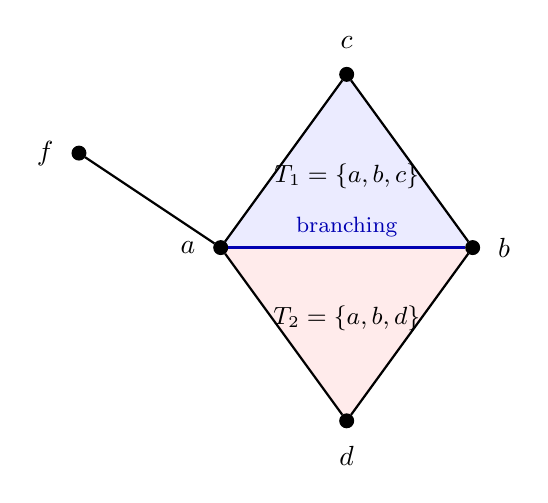
\begin{tikzpicture}[
  vertex/.style={circle, draw, fill=black, inner sep=1.5pt, minimum size=5pt},
  edge/.style={thick},
  branchedge/.style={very thick, blue!70!black},
  triA/.style={fill=blue!8},
  triB/.style={fill=red!8},
  label distance=3pt
]
  % Vertices
  \node[vertex, label=left:$a$]  (a) at (0,0) {};
  \node[vertex, label=right:$b$] (b) at (3.2,0) {};
  \node[vertex, label=above:$c$] (c) at (1.6,2.2) {};
  \node[vertex, label=below:$d$] (d) at (1.6,-2.2) {};
  \node[vertex, label=left:$f$]  (f) at (-1.8,1.2) {};

  % Filled triangles
  \begin{scope}[on background layer]
    \fill[triA] (a.center) -- (b.center) -- (c.center) -- cycle;
    \fill[triB] (a.center) -- (b.center) -- (d.center) -- cycle;
  \end{scope}

  % Edges
  \draw[branchedge] (a) -- (b) node[midway, above, font=\footnotesize,
    text=blue!70!black] {branching};
  \draw[edge] (a) -- (c);
  \draw[edge] (b) -- (c);
  \draw[edge] (a) -- (d);
  \draw[edge] (b) -- (d);
  \draw[edge] (a) -- (f);

  % Triangle labels
  \node[font=\small] at (1.6,0.9) {$T_1 = \{a,b,c\}$};
  \node[font=\small] at (1.6,-0.9) {$T_2 = \{a,b,d\}$};

\end{tikzpicture}
\caption{A finite nerve with five vertices, six edges, and two triangles.
The edge~$\{a,b\}$ is a \emph{branching edge}: it is a codimension-one face
of both~$T_1$ and~$T_2$. The vertex~$f$ is connected only to~$a$; the edge
$\{a,f\}$ is neither triangle-bearing nor branching.}
\label{fig:nerve}
\end{figure}

\begin{example}
\label{ex:nerve}
Figure~\ref{fig:nerve} shows a nerve~$\cN$ with vertex set
$I = \{a,b,c,d,f\}$. The nerve has two triangles, $T_1 = \{a,b,c\}$ and
$T_2 = \{a,b,d\}$, which share the branching edge~$\{a,b\}$.
The remaining edges~$\{a,c\}$, $\{b,c\}$, $\{a,d\}$, $\{b,d\}$ are
triangle-bearing but not branching (each belongs to exactly one triangle).
The edge~$\{a,f\}$ is not triangle-bearing.
\end{example}

% ============================================================
\section{Orientation data and boundary operators}
\label{sec:orientation}
% ============================================================

To define boundary operators on an abstract simplicial complex whose
simplices are \emph{unordered} finite sets, one must introduce auxiliary
\emph{orientation data} that assign an ordering to the vertices of each
simplex. We recall the standard construction (cf.~\cite[Chapter~2]{Hatcher:2002},
\cite[Chapter~1]{Munkres:1984}) and adapt it to the finite nerve setting.

\begin{definition}[Ordered witness]
\label{def:witness}
An \emph{ordered witness} of a $k$-simplex~$\sigma = \{v_0, \ldots, v_k\}
\in \cN_k$ is a bijection $w \colon \{0, \ldots, k\} \to \sigma$.
We write~$w = (w(0), w(1), \ldots, w(k))$ as an ordered tuple.
\end{definition}

For a $1$-simplex~$e = \{a,b\}$, the two ordered witnesses are~$(a,b)$
and~$(b,a)$. For a $2$-simplex~$\sigma = \{a,b,c\}$, there are six
ordered witnesses, corresponding to the six permutations of~$\{a,b,c\}$.

\begin{definition}[Induced edge boundary]
\label{def:edge-boundary}
Given an ordered witness~$w = (v_0, v_1)$ of an edge~$e \in \cN_1$,
the \emph{induced boundary} is
\begin{equation}
  \label{eq:edge-boundary}
  \partial_1 [v_0, v_1] \;=\; [v_1] - [v_0]\,.
\end{equation}
In matrix form, the boundary operator~$\partial_1$ is the
$|\cN_0| \times |\cN_1|$ matrix over~$\ZZ$ with entries
\[
  (\partial_1)_{v,e} =
  \begin{cases}
    +1 & \text{if } v = w(1) \text{ (the positive vertex)}, \\
    -1 & \text{if } v = w(0) \text{ (the negative vertex)}, \\
    \;0 & \text{if } v \notin e.
  \end{cases}
\]
\end{definition}

\begin{definition}[Induced triangle boundary]
\label{def:triangle-boundary}
Given an ordered witness~$w = (v_0, v_1, v_2)$ of a triangle~$\sigma
\in \cN_2$, the \emph{induced boundary} is
\begin{equation}
  \label{eq:triangle-boundary}
  \partial_2 [v_0, v_1, v_2] \;=\; [v_1, v_2] - [v_0, v_2] + [v_0, v_1]\,.
\end{equation}
More precisely, each boundary edge of~$\sigma$ inherits an orientation:
the edge obtained by removing the vertex~$v_j$ receives the sign~$(-1)^j$.
\end{definition}

\begin{definition}[Positional edge and chosen face]
\label{def:chosen-face}
Let~$w = (w_0, w_1, w_2)$ be an ordered witness of a triangle
$\sigma \in \cN_2$. For $0 \leq p < q \leq 2$, the \emph{$pq$-edge}
of~$w$ is the edge~$\{w_p, w_q\} \in \cN_1$.
Each boundary edge~$e$ of~$\sigma$ is the $pq$-edge of~$w$ for a unique
pair~$p < q$, since the three boundary edges are
$\{w_0,w_1\}$, $\{w_0,w_2\}$, and~$\{w_1,w_2\}$.

The \emph{chosen face} of a boundary edge~$e = \{w_p, w_q\}$ (with $p < q$)
relative to~$w$ is the codimension-one face~$\{w_q\}$ of the edge ---
the vertex occupying the later position in the witness tuple. We write
\[
  \chosenface_w(e) = \{w_q\}\,.
\]
Equivalently, $\chosenface_w(e)$ is the vertex of~$e$ with positive
coefficient in the boundary~$\partial_1[w_p, w_q] = [w_q] - [w_p]$.
\end{definition}

\begin{example}
\label{ex:chosen}
For the triangle~$\sigma = \{a,b,c\}$ with witness~$w = (a,b,c)$:
\begin{itemize}[nosep]
  \item $\chosenface_w(\{a,b\}) = \{b\}$
        \quad (from the ordering $(a,b)$, second vertex is~$b$),
  \item $\chosenface_w(\{a,c\}) = \{c\}$
        \quad (from the ordering $(a,c)$, second vertex is~$c$),
  \item $\chosenface_w(\{b,c\}) = \{c\}$
        \quad (from the ordering $(b,c)$, second vertex is~$c$).
\end{itemize}
Under the transposition~$\swapAB(w) = (b,a,c)$, the edge~$\{a,b\}$
inherits the ordering~$(b,a)$, so the chosen face becomes
$\chosenface_{\swapAB(w)}(\{a,b\}) = \{a\} \neq \{b\}$.
\end{example}

\begin{definition}[Global orientation data]
\label{def:global-orientation}
A \emph{global edge orientation datum} is a function assigning to each
edge~$e \in \cN_1$ an ordered witness of~$e$.
A \emph{global triangle witness datum} is a function~$\cT$ assigning to
each triangle~$\sigma \in \cN_2$ an ordered witness~$\cT(\sigma)$ of~$\sigma$.
\end{definition}

Given global orientation data, the boundary operators~$\partial_1$
and~$\partial_2$ are the integer matrices defined by applying
Definitions~\ref{def:edge-boundary} and~\ref{def:triangle-boundary}
to each simplex using its assigned ordered witness.

% ============================================================
\section{Compatibility and the chain complex}
\label{sec:chain-complex}
% ============================================================

The chain complex property~$\partial_1 \circ \partial_2 = 0$ does not
hold for arbitrary orientation data. It requires a \emph{compatibility
condition} relating the edge orientations to the triangle witnesses.

\begin{definition}[Compatibility]
\label{def:compatibility}
Let $\omega_1$ be a global edge orientation datum and $\omega_2$ a global
triangle witness datum. We say that~$(\omega_1, \omega_2)$ are
\emph{compatible} if, for every vertex~$v \in \cN_0$ and every
triangle~$\sigma \in \cN_2$, the three signed contributions from the
boundary edges of~$\sigma$ to the vertex~$v$ cancel:
\begin{equation}
  \label{eq:composition-entry}
  \sum_{e \in \cN_1} (\partial_1)_{v, e}\, (\partial_2)_{e, \sigma}
  \;=\; 0\,.
\end{equation}
Since~$(\partial_2)_{e,\sigma} \neq 0$ only when~$e$ is a boundary edge
of~$\sigma$, and each triangle has exactly three boundary edges, the sum
has at most three nonzero terms.
\end{definition}

\begin{theorem}[Chain complex]
\label{thm:chain-complex}
Let~$\cN$ be a finite nerve, and let~$(\omega_1, \omega_2)$ be compatible
global orientation data. Then:
\begin{enumerate}[label=\textup{(\roman*)},nosep]
  \item The composition vanishes:~$\partial_1 \circ \partial_2 = 0$
        as a matrix over~$\ZZ$.
  \item Every $1$-boundary is a $1$-cycle: $\operatorname{im} \partial_2
        \subseteq \ker \partial_1$, i.e., $B_1 \leq Z_1$.
  \item The first homology group
        \[
          H_1 \;=\; Z_1 / B_1
          \;=\; \ker \partial_1 \,/\, \operatorname{im} \partial_2
        \]
        is a well-defined finitely generated abelian group.
\end{enumerate}
\end{theorem}

\begin{proof}[Proof sketch]
Part~(i): the $(v, \sigma)$-entry of~$\partial_1 \circ \partial_2$ is
exactly the sum in~\eqref{eq:composition-entry}, which vanishes by the
compatibility condition. Since this holds for all~$(v,\sigma)$, the
entire matrix is zero. Part~(ii) follows from~(i): if
$z = \partial_2 c$ for some $2$-chain~$c$, then
$\partial_1 z = (\partial_1 \circ \partial_2) c = 0$.
Part~(iii) is a standard algebraic consequence of~(ii).
\end{proof}

The compatibility condition can equivalently be expressed in terms of a
\emph{local orientation datum}. A local orientation datum assigns to each
simplex a consistent labeling of its codimension-one faces. The key
equivalence is:

\begin{proposition}[Compatibility equivalence]
\label{prop:compat-equiv}
A global edge orientation datum~$\omega_1$ and a global triangle witness
datum~$\omega_2$ are compatible if and only if there exists a
\emph{boundary local orientation datum}~$\theta$ --- a function assigning
to each simplex a consistent labeling of its codimension-one faces ---
such that~$\omega_1$ and~$\omega_2$ are both induced from~$\theta$.
\end{proposition}

\begin{proof}[Proof sketch]
The forward direction constructs~$\theta$ from~$(\omega_1, \omega_2)$ by
reading off the sign assignments on codimension-one faces from the
boundary matrices. The converse verifies that if~$\omega_1$ and~$\omega_2$
are both induced from a single~$\theta$, then for each vertex~$v$
and each triangle~$\sigma = [v_0, v_1, v_2]$ the sum
$\sum_{j=0}^{2} (-1)^j (\partial_1)_{v,\, [v_0, \ldots, \hat{v}_j,
\ldots, v_2]}$ vanishes, which is the standard boundary-of-boundary
cancellation.
See the Lean module \texttt{BoundaryCompatibilityEquiv} for the full proof.
\end{proof}

% ============================================================
\section{Existence of compatible orientation data}
\label{sec:existence}
% ============================================================

We now show that compatible orientation data always exist. The construction
proceeds in two steps: first, one assigns an ordered witness to each
triangle; second, one derives compatible edge orientations from the
triangle witnesses.

\begin{definition}[Edge-triangle choice compatibility]
\label{def:edge-triangle-compat}
Let~$\chi$ be a global edge orientation datum and~$\cT$ a global
triangle witness datum. We say that~$(\chi, \cT)$ are
\emph{globally choice-compatible} if, for every triangle
$\sigma \in \cN_2$ and every boundary edge~$e$ of~$\sigma$, the
edge orientation assigned by~$\chi$ agrees with the orientation
induced on~$e$ by the triangle witness~$\cT(\sigma)$.
\end{definition}

\begin{construction}[Compatible data from triangle witnesses]
\label{con:from-witnesses}
Let~$\cT$ be a global triangle witness datum satisfying a
\emph{coherence condition} (to be defined in Section~\ref{sec:coherence}).
For each edge~$e \in \cN_1$:
\begin{itemize}[nosep]
  \item If~$e$ is a boundary edge of some triangle~$\sigma$, define the
        edge orientation of~$e$ to be the one induced by~$\cT(\sigma)$.
        The coherence condition ensures that this is independent of the
        choice of~$\sigma$.
  \item If~$e$ is not triangle-bearing, assign an arbitrary orientation
        to~$e$.
\end{itemize}
This produces a globally choice-compatible pair~$(\chi, \cT)$.
\end{construction}

\begin{proposition}
\label{prop:coherent-exists}
For any finite nerve~$\cN$, there exists a global triangle witness
datum~$\cT$ satisfying the coherence condition of
Definition~\ref{def:coherence}.
\end{proposition}

\begin{proof}[Proof sketch]
Choose any total order~$\leq$ on the vertex set~$I$. For each triangle
$\sigma = \{i,j,k\}$ with~$i < j < k$, set $\cT(\sigma) = (i,j,k)$.
The resulting datum is coherent because any two triangles sharing an
edge~$\{i,j\}$ both place~$i$ before~$j$, hence agree on the chosen
face~$\{j\}$. This construction is noncanonical: it depends on the
choice of total order on~$I$.
\end{proof}

\begin{theorem}[Existence]
\label{thm:existence}
For any finite nerve~$\cN$, there exist compatible orientation data
$(\omega_1, \omega_2)$ such that~$\partial_1 \circ \partial_2 = 0$.
\end{theorem}

\begin{proof}
Take a coherent global witness datum~$\cT$ from
Proposition~\ref{prop:coherent-exists} and apply
Construction~\ref{con:from-witnesses} to obtain a globally
choice-compatible pair~$(\omega_1, \omega_2)$. Coherence ensures
that the edge orientation on every triangle-bearing edge is
well-defined, and direct verification of~\eqref{eq:composition-entry}
for each~$(v, \sigma)$ then gives~$\partial_1 \circ \partial_2 = 0$.
\end{proof}

\begin{remark}
\label{rem:noncanonical}
The key point is that the existence proof uses a total order on the
vertex set, which is \emph{not part of the nerve data}. The nerve
structure provides only the unordered simplices. Whether a canonical
total order can be derived from richer structural data (such as a
partial order on the underlying space) is an open question; see
Section~\ref{sec:discussion}.
\end{remark}

% ============================================================
\section{Coherence conditions and their equivalences}
\label{sec:coherence}
% ============================================================

The compatibility of Construction~\ref{con:from-witnesses} requires that
all triangle witnesses on a shared edge agree on the induced edge
orientation. We now make this precise and establish several equivalent
formulations.

\begin{definition}[Pairwise branching coherence]
\label{def:coherence}
Let~$\cT$ be a global triangle witness datum. We say that~$\cT$
satisfies \emph{pairwise branching chosen-face coherence} if, for every
branching edge~$e \in \cN_1$ and every pair of triangles~$\sigma_1,
\sigma_2 \in \cN_2$ having~$e$ as a codimension-one face, the chosen faces
agree:
\[
  \chosenface_{\cT(\sigma_1)}(e)
  \;=\; \chosenface_{\cT(\sigma_2)}(e)\,.
\]
\end{definition}

\begin{definition}[Branching-edge conflict]
\label{def:conflict}
A \emph{branching-edge conflict} for a global witness datum~$\cT$ is a
branching edge~$e$ and two triangles~$\sigma_1, \sigma_2$ having~$e$ as
a face, such that the induced local edge orientations disagree:
\[
  \chosenface_{\cT(\sigma_1)}(e)
  \;\neq\; \chosenface_{\cT(\sigma_2)}(e)\,.
\]
\end{definition}

\begin{proposition}[Conflict--coherence duality]
\label{prop:conflict-iff}
A global witness datum~$\cT$ satisfies pairwise branching coherence if
and only if it has no branching-edge conflict.
\end{proposition}

\begin{proof}
Immediate from the definitions: coherence is the negation of a conflict
at every branching edge.
\end{proof}

The coherence condition admits several equivalent formulations, each
illuminating a different aspect:

\begin{theorem}[Equivalence of coherence conditions]
\label{thm:equiv}
Let~$\cT$ be a global triangle witness datum. The following are equivalent:
\begin{enumerate}[label=\textup{(\roman*)},nosep]
  \item \emph{Pairwise branching coherence:}
        all triangle witnesses on each branching edge induce the same
        chosen face.
  \item \emph{Glued branching-edge choices:}
        there exists a function assigning to each branching edge a chosen
        face, consistent with all adjacent triangle witnesses.
  \item \emph{Pure triangle-overlap coherence:}
        for every pair of distinct triangles sharing a codimension-one face,
        the induced local edge orientations on the shared edge agree.
  \item \emph{Global edge-orientation coherence:}
        the triangle witnesses induce a well-defined global edge orientation
        on every triangle-bearing edge.
\end{enumerate}
\end{theorem}

\begin{proof}[Proof sketch]
The implications (ii)$\Rightarrow$(i) and (i)$\Rightarrow$(iii)
follow by unwinding the definitions.
The implication (iii)$\Rightarrow$(ii) uses the fact that on each
branching edge, the pairwise agreement of all triangle witnesses implies
the existence of a single consistent chosen face.
The equivalence (i)$\Leftrightarrow$(iv) follows from the observation
that the local edge orientation is determined by the chosen face
(via~\eqref{eq:edge-boundary}), and conversely, the chosen face is
recovered from the orientation. Complete proofs are in the Lean
formalization; see Appendix~\ref{app:lean}.
\end{proof}

\begin{corollary}
\label{cor:coherence-implies-compat}
If a global witness datum~$\cT$ satisfies pairwise branching coherence,
then there exist compatible orientation data~$(\omega_1, \omega_2)$
with~$\partial_1 \circ \partial_2 = 0$, where~$\omega_2$ is
determined by~$\cT$ and~$\omega_1$ is the induced global edge
orientation.
\end{corollary}

\begin{proof}
Apply Construction~\ref{con:from-witnesses} to derive~$\omega_1$
from~$\cT$: the coherence condition (Definition~\ref{def:coherence})
guarantees that the induced edge orientation is well-defined on every
triangle-bearing edge. The resulting pair~$(\omega_1, \omega_2)$ is
globally choice-compatible (Definition~\ref{def:edge-triangle-compat}),
which implies compatibility (Definition~\ref{def:compatibility}).
\end{proof}

\begin{remark}[Same nerve, different orderings]
\label{rem:same-support}
Since a global witness datum is a function defined on all
of~$\cN_2$, any two global witness data on the same nerve~$\cN$
are automatically defined on the same domain of triangles.
They can differ only in the \emph{vertex orderings} assigned to
individual triangles, not in which triangles receive witnesses.
When we say that~$\cT$ and~$\cT'$ ``have the same simplicial
support,'' we mean precisely this: they are global witness data
on the same nerve.
\end{remark}

% ============================================================
\section{The non-intrinsicness obstruction}
\label{sec:obstruction}
% ============================================================

We now prove the main negative result: the coherence condition of
Section~\ref{sec:coherence} is not a property of the simplicial support
data of the nerve. It depends on the specific ordered witnesses assigned
to each triangle, and different witness choices on the same simplicial
support can lead to mutually exclusive coherence outcomes.

\subsection{Vertex transpositions on triangle witnesses}
\label{sec:swaps}

\begin{definition}[Vertex transpositions]
\label{def:swaps}
Let~$w = (v_0, v_1, v_2)$ be an ordered witness of a triangle~$\sigma$.
We define three transposition operations:
\begin{align}
  \swapAB(w) &= (v_1, v_0, v_2)\,, \label{eq:swapAB} \\
  \swapAC(w) &= (v_2, v_1, v_0)\,, \label{eq:swapAC} \\
  \swapBC(w) &= (v_0, v_2, v_1)\,. \label{eq:swapBC}
\end{align}
Each transposition produces a valid ordered witness of the same
underlying triangle~$\sigma$.
\end{definition}

The key observation is that transpositions preserve the underlying edge
but change the chosen face:

\begin{lemma}[Edge preservation]
\label{lem:edge-preservation}
Let~$w = (v_0, v_1, v_2)$. Then:
\begin{enumerate}[label=\textup{(\alph*)},nosep]
  \item $\swapAB(w)$ preserves the $01$-edge
        (Definition~\ref{def:chosen-face}): both~$w$ and~$\swapAB(w)$
        have~$\{v_0, v_1\}$ as their $01$-edge.
  \item $\swapAC(w)$ preserves the $02$-edge $\{v_0, v_2\}$.
  \item $\swapBC(w)$ preserves the $12$-edge $\{v_1, v_2\}$.
\end{enumerate}
\end{lemma}

\begin{proof}
In each case, the transposition exchanges two vertices of the edge,
which preserves the edge as an unordered set.
\end{proof}

\begin{theorem}[Witness flexibility]
\label{thm:flexibility}
Let~$w = (v_0, v_1, v_2)$ be an ordered witness. The following hold:
\begin{enumerate}[label=\textup{(\alph*)},nosep]
  \item $\chosenface_w(\{v_0, v_1\}) \neq
        \chosenface_{\swapAB(w)}(\{v_0, v_1\})$.
  \item $\chosenface_w(\{v_0, v_2\}) \neq
        \chosenface_{\swapAC(w)}(\{v_0, v_2\})$.
  \item $\chosenface_w(\{v_1, v_2\}) \neq
        \chosenface_{\swapBC(w)}(\{v_1, v_2\})$.
\end{enumerate}
That is, each transposition flips the chosen face on the preserved edge.
\end{theorem}

\begin{proof}
We prove (a); the arguments for (b) and (c) are identical.
Under~$w = (v_0, v_1, v_2)$, the edge~$\{v_0, v_1\}$ inherits the
ordering~$(v_0, v_1)$, so $\chosenface_w(\{v_0, v_1\}) = \{v_1\}$.
Under~$\swapAB(w) = (v_1, v_0, v_2)$, the same edge inherits the
ordering~$(v_1, v_0)$, so
$\chosenface_{\swapAB(w)}(\{v_0, v_1\}) = \{v_0\}$.
Since~$v_0 \neq v_1$ (the vertices of an edge are distinct),
$\{v_1\} \neq \{v_0\}$.
\end{proof}

\subsection{The main obstruction theorem}
\label{sec:main-theorem}

We now lift the single-triangle witness flexibility to a global statement
about pairs of triangles sharing a branching edge.

\begin{definition}[Witness replacement]
\label{def:replacement}
Let~$\cT$ be a global triangle witness datum. For a triangle~$\sigma$
and an ordered witness~$w$ of~$\sigma$, we write~$\cT[\sigma \leftarrow w]$
for the global datum that agrees with~$\cT$ on all triangles except~$\sigma$,
where it assigns~$w$ instead.
\end{definition}

\begin{theorem}[Non-intrinsicness obstruction]
\label{thm:main-obstruction}
Let~$\cN$ be a finite nerve. Let~$T_1 \neq T_2 \in \cN_2$ be distinct
triangles sharing a boundary edge~$e$. Let~$w_1$ be an ordered witness
of~$T_1$ and~$w_2$ an ordered witness of~$T_2$ such that~$e$ is the
$01$-edge of both~$w_1$ and~$w_2$. For any base global witness
datum~$\cT_0$, define:
\begin{align}
  \cT &\;=\; \cT_0[T_1 \leftarrow w_1][T_2 \leftarrow w_2]\,,
  \label{eq:tau} \\
  \cT' &\;=\; \cT_0[T_1 \leftarrow w_1][T_2 \leftarrow \swapAB(w_2)]\,.
  \label{eq:tau-swap}
\end{align}
Then:
\begin{enumerate}[label=\textup{(\alph*)},nosep]
  \item\label{item:not-both}
    $\cT$ and~$\cT'$ cannot both satisfy pairwise branching coherence
    on the edge~$e$:
    \[
      \neg\bigl(\text{$\cT$ coherent at $e$}
      \;\wedge\;
      \text{$\cT'$ coherent at $e$}\bigr)\,.
    \]
  \item\label{item:conditional}
    If~$\cT$ satisfies pairwise branching coherence at~$e$, then~$\cT'$
    has a branching-edge conflict at~$e$.
  \item\label{item:global}
    $\cT$ and~$\cT'$ cannot both satisfy \emph{global} pairwise
    branching coherence:
    \[
      \neg\bigl(\text{$\cT$ globally coherent}
      \;\wedge\;
      \text{$\cT'$ globally coherent}\bigr)\,.
    \]
\end{enumerate}
\end{theorem}

\begin{proof}
Since~$T_1 \neq T_2$ and both have~$e$ as a codimension-one face,
$e$ is a branching edge.
Write~$w_2 = (w_2^{(0)}, w_2^{(1)}, w_2^{(2)})$. By hypothesis,
$e = \{w_2^{(0)}, w_2^{(1)}\}$ is the $01$-edge of~$w_2$.

\medskip\noindent\textit{Key observation.}
By Definition~\ref{def:chosen-face}:
\begin{align*}
  \chosenface_{w_2}(e) &= \{w_2^{(1)}\}\,,\\
  \chosenface_{\swapAB(w_2)}(e) &= \{w_2^{(0)}\}\,.
\end{align*}
The second equality holds because~$\swapAB(w_2)
= (w_2^{(1)}, w_2^{(0)}, w_2^{(2)})$ has the same underlying edge
$\{w_2^{(1)}, w_2^{(0)}\} = e$, but with the positions swapped, so the
vertex in the later position is now~$w_2^{(0)}$.
Since~$w_2^{(0)} \neq w_2^{(1)}$ (the vertices of an edge are distinct):
\begin{equation}
  \label{eq:two-faces-differ}
  \chosenface_{w_2}(e) \;\neq\; \chosenface_{\swapAB(w_2)}(e)\,.
\end{equation}

\medskip\noindent\textit{Proof of~\ref{item:not-both}.}
Under~$\cT$, the witnesses on~$T_1$ and~$T_2$ induce chosen faces
$\chosenface_{w_1}(e)$ and $\chosenface_{w_2}(e)$ on the shared edge~$e$.
Under~$\cT'$, they induce $\chosenface_{w_1}(e)$ and
$\chosenface_{\swapAB(w_2)}(e)$.
Coherence at~$e$ for~$\cT$ requires
$\chosenface_{w_1}(e) = \chosenface_{w_2}(e)$;
coherence at~$e$ for~$\cT'$ requires
$\chosenface_{w_1}(e) = \chosenface_{\swapAB(w_2)}(e)$.
By~\eqref{eq:two-faces-differ}, the right-hand sides are distinct,
so~$\chosenface_{w_1}(e)$ cannot equal both.

\medskip\noindent\textit{Proof of~\ref{item:conditional}.}
If~$\cT$ is coherent at~$e$, then
$\chosenface_{w_1}(e) = \chosenface_{w_2}(e) \neq
\chosenface_{\swapAB(w_2)}(e)$, so~$\cT'$ has a conflict at~$e$
(Definition~\ref{def:conflict}).

\medskip\noindent\textit{Proof of~\ref{item:global}.}
Global coherence implies local coherence at every branching edge,
including~$e$, so~\ref{item:global} follows from~\ref{item:not-both}.
\end{proof}

\begin{figure}[t]
\centering
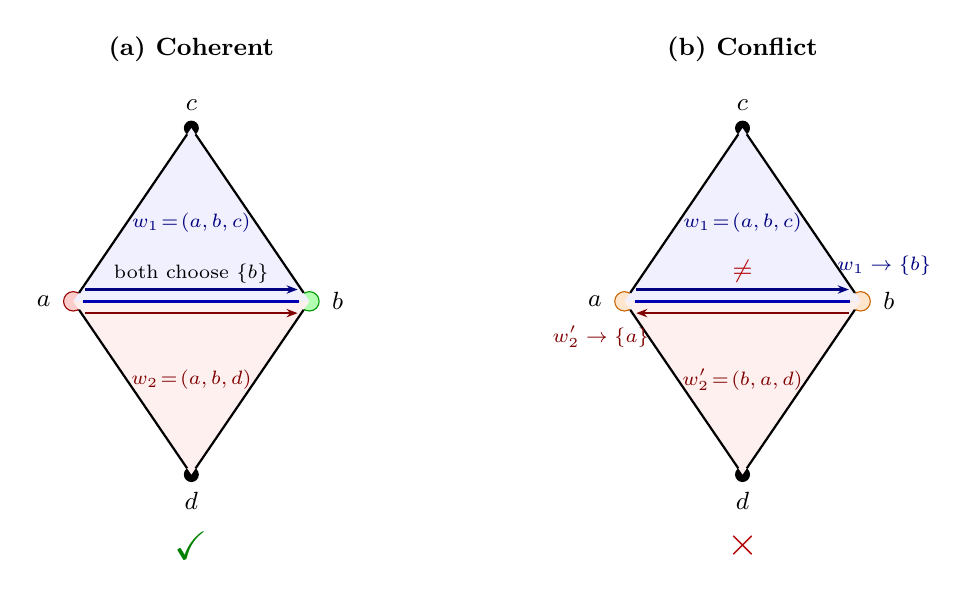
\begin{tikzpicture}[
  vertex/.style={circle, draw, fill=black, inner sep=1.5pt, minimum size=5pt},
  posvertex/.style={circle, draw=green!60!black, fill=green!30,
    inner sep=1.5pt, minimum size=7pt},
  negvertex/.style={circle, draw=red!60!black, fill=red!20,
    inner sep=1.5pt, minimum size=7pt},
  edge/.style={thick},
  branchedge/.style={very thick, blue!70!black},
  checkmark/.style={font=\Large},
  panel/.style={font=\bfseries\small}
]
  % === Panel (a): Coherent ===
  \begin{scope}[shift={(0,0)}]
    \node[panel] at (1.5,3.2) {(a) Coherent};

    % Vertices
    \node[posvertex, label={[label distance=1pt]right:\small$b$}]
      (a-b) at (3,0) {};
    \node[negvertex, label={[label distance=1pt]left:\small$a$}]
      (a-a) at (0,0) {};
    \node[vertex, label=above:\small$c$] (a-c) at (1.5,2.2) {};
    \node[vertex, label=below:\small$d$] (a-d) at (1.5,-2.2) {};

    % Triangles
    \fill[blue!6] (a-a.center) -- (a-b.center) -- (a-c.center) -- cycle;
    \fill[red!6]  (a-a.center) -- (a-b.center) -- (a-d.center) -- cycle;

    % Edges
    \draw[branchedge] (a-a) -- (a-b);
    \draw[edge] (a-a) -- (a-c); \draw[edge] (a-b) -- (a-c);
    \draw[edge] (a-a) -- (a-d); \draw[edge] (a-b) -- (a-d);

    % Witness arrows
    \draw[-{Stealth[length=4pt]}, thick, blue!50!black]
      ($(a-a)+(0.15,0.15)$) -- ($(a-b)+(-0.15,0.15)$);
    \draw[-{Stealth[length=4pt]}, thick, red!50!black]
      ($(a-a)+(0.15,-0.15)$) -- ($(a-b)+(-0.15,-0.15)$);

    % Labels
    \node[font=\scriptsize, blue!50!black] at (1.5, 1.0)
      {$w_1\!=\!(a,b,c)$};
    \node[font=\scriptsize, red!50!black] at (1.5, -1.0)
      {$w_2\!=\!(a,b,d)$};
    \node[font=\scriptsize] at (1.5, 0.35)
      {both choose $\{b\}$};

    % Checkmark
    \node[checkmark, green!50!black] at (1.5, -3.1) {\checkmark};
  \end{scope}

  % === Panel (b): Conflict ===
  \begin{scope}[shift={(7,0)}]
    \node[panel] at (1.5,3.2) {(b) Conflict};

    % Vertices — both highlighted as contested
    \node[vertex, draw=orange!80!black, fill=orange!20,
      inner sep=1.5pt, minimum size=7pt,
      label={[label distance=1pt]right:\small$b$}]
      (b-b) at (3,0) {};
    \node[vertex, draw=orange!80!black, fill=orange!20,
      inner sep=1.5pt, minimum size=7pt,
      label={[label distance=1pt]left:\small$a$}]
      (b-a) at (0,0) {};
    \node[vertex, label=above:\small$c$] (b-c) at (1.5,2.2) {};
    \node[vertex, label=below:\small$d$] (b-d) at (1.5,-2.2) {};

    % Triangles
    \fill[blue!6] (b-a.center) -- (b-b.center) -- (b-c.center) -- cycle;
    \fill[red!6]  (b-a.center) -- (b-b.center) -- (b-d.center) -- cycle;

    % Edges
    \draw[branchedge] (b-a) -- (b-b);
    \draw[edge] (b-a) -- (b-c); \draw[edge] (b-b) -- (b-c);
    \draw[edge] (b-a) -- (b-d); \draw[edge] (b-b) -- (b-d);

    % Witness arrows (T1 same, T2 reversed)
    \draw[-{Stealth[length=4pt]}, thick, blue!50!black]
      ($(b-a)+(0.15,0.15)$) -- ($(b-b)+(-0.15,0.15)$);
    \draw[-{Stealth[length=4pt]}, thick, red!50!black]
      ($(b-b)+(-0.15,-0.15)$) -- ($(b-a)+(0.15,-0.15)$);

    % Labels
    \node[font=\scriptsize, blue!50!black] at (1.5, 1.0)
      {$w_1\!=\!(a,b,c)$};
    \node[font=\scriptsize, red!50!black] at (1.5, -1.0)
      {$w_2'\!=\!(b,a,d)$};

    % Conflict annotation: each label near the CHOSEN vertex
    \node[font=\scriptsize, blue!50!black] at (3.3, 0.45)
      {$w_1 \to \{b\}$};
    \node[font=\scriptsize, red!50!black] at (-0.3, -0.45)
      {$w_2' \to \{a\}$};
    \node[font=\small, red!70!black] at (1.5, 0.38)
      {$\neq$};

    % Cross
    \node[checkmark, red!70!black] at (1.5, -3.1) {$\times$};
  \end{scope}
\end{tikzpicture}
\caption{The witness-swap obstruction on a shared branching edge
$e = \{a,b\}$. \textbf{(a)}~Both triangle witnesses~$(a,b,c)$
and~$(a,b,d)$ induce the same chosen face~$\{b\}$ (green vertex) on~$e$:
the datum is coherent. \textbf{(b)}~After applying~$\swapAB$ to the
witness on~$T_2$, the witness becomes~$(b,a,d)$ and the chosen face
on~$e$ flips to~$\{a\}$. Since~$w_1$ still chooses~$\{b\}$, the
datum has a conflict. By Theorem~\ref{thm:main-obstruction},
$\cT$~and~$\cT'$ cannot both be coherent.}
\label{fig:obstruction}
\end{figure}

\begin{corollary}[Non-intrinsicness]
\label{cor:non-intrinsic}
The global coherence condition (Definition~\ref{def:coherence}) is not
determined by the simplicial support of the nerve. Specifically, there
exist global witness data~$\cT$ and~$\cT'$ with the same underlying
simplicial support (the same set of triangles, as unordered sets) but
different coherence status.
\end{corollary}

\begin{proof}
Take any nerve with a branching edge, choose triangles~$T_1 \neq T_2$
sharing the branching edge, and construct~$\cT$ and~$\cT'$ as in
Theorem~\ref{thm:main-obstruction}. The data~$\cT$ and~$\cT'$ agree
on every triangle except~$T_2$, where they assign different ordered
witnesses of the \emph{same unordered triangle}. Thus the simplicial
support is identical. By Theorem~\ref{thm:main-obstruction},
at most one of~$\cT$ and~$\cT'$ can be coherent.
\end{proof}

\begin{remark}
\label{rem:not-impossibility}
Theorem~\ref{thm:main-obstruction} does \emph{not} assert that no
coherent global witness datum exists. It asserts that coherence is
not a property of the simplicial support: among witness data with the
same support, the coherent ones form a proper subset that depends on the
ordering choices. Proposition~\ref{prop:coherent-exists} confirms that
coherent data do exist (using a total vertex order).
\end{remark}

\begin{remark}
\label{rem:all-edges}
The obstruction is uniform across all three boundary edges.
Theorem~\ref{thm:flexibility} shows that~$\swapAB$, $\swapAC$,
and~$\swapBC$ each flip the chosen face on their respective preserved
edges. Thus the non-intrinsicness is not an artifact of a particular
edge labeling.
\end{remark}

\begin{remark}[Localization]
\label{rem:localization}
Parts~\ref{item:conditional} and~\ref{item:global} of
Theorem~\ref{thm:main-obstruction} show that the obstruction is
\emph{one-sided and localized}: if one of the two witness data is
globally coherent, the other carries a conflict on the very same
branching edge where the transposition was performed.
\end{remark}

% ============================================================
\section{Discussion}
\label{sec:discussion}
% ============================================================

\subsection{Summary of results}

We have established two complementary results about boundary operators
on finite nerves:

\begin{enumerate}[nosep]
  \item \emph{Auxiliary construction works.}
    Given a global triangle witness datum satisfying pairwise branching
    coherence, the induced boundary operators form a chain complex
    with~$\partial_1 \circ \partial_2 = 0$ and well-defined first
    homology~$H_1$ (Theorem~\ref{thm:chain-complex}).
    Compatible data always exist (Theorem~\ref{thm:existence}),
    but their construction is noncanonical.

  \item \emph{Intrinsic coherence from support data alone fails.}
    The coherence condition that ensures compatibility is not determined
    by the simplicial support of the nerve
    (Corollary~\ref{cor:non-intrinsic}).
    Two witness data on the same support, differing by a single vertex
    transposition, cannot both be coherent
    (Theorem~\ref{thm:main-obstruction}).
    This obstruction is localized to branching edges, is uniform across
    all three boundary edges, and admits both disjunctive and
    conditional forms.
\end{enumerate}

\subsection{Implications for the spectral action program}

In the context of spectral causal theory, the question motivating this
work asks whether the combinatorial data of a finite
approximation to spacetime suffice to define boundary operators and
homological invariants intrinsically. Our results show that the
\emph{nerve structure alone is insufficient}: the unordered simplicial
support does not determine the needed orientation data.

This does not close the broader problem. Three directions remain open:

\begin{enumerate}[nosep]
  \item \emph{The causal order escape route.}
    A finite causal set carries a partial order that is strictly richer
    than the nerve support data. This partial order could in principle
    provide a canonical source of vertex orderings (e.g., by extending
    the partial order to a total order and using it to orient all
    simplices). The Lean formalization works with abstract covers and
    nerves without reference to partial orders, so
    Theorem~\ref{thm:main-obstruction} does not address this possibility.

  \item \emph{Weaker reconstruction goals.}
    Boundary operators over~$\ZZ/2\ZZ$ do not require orientations:
    the unsigned incidence matrices already define a chain complex
    over~$\ZZ/2\ZZ$. The resulting mod-$2$ homology is intrinsic to
    the nerve support. However, integer-valued homology is needed for
    most physical applications (orientation, characteristic classes,
    the spectral action functional).

  \item \emph{Ensemble and emergent approaches.}
    One may weaken the demand from intrinsic reconstruction on a single
    nerve to statistical emergence from an ensemble of nerves, or allow
    the spectral triple to be defined only after a coarse-graining step.
    These approaches relax the directness of the reconstruction but
    may circumvent the obstruction.
\end{enumerate}

\subsection{Relation to classical orientation theory}

The non-intrinsicness of orientation data on simplicial complexes is
a well-known phenomenon in algebraic topology
(cf.~\cite{Hatcher:2002,Munkres:1984}). Every abstract simplicial
complex admits orientations (by choosing a total vertex order), but the
orientation is not part of the combinatorial data. Two key differences
between the classical setting and the present one are:

\begin{itemize}[nosep]
  \item In classical simplicial homology, the homology groups are
        independent of the choice of orientation (up to isomorphism).
        In the present setting, coherent data always exist
        (Proposition~\ref{prop:coherent-exists}), but \emph{whether
        a particular witness datum is coherent} depends on the specific
        vertex orderings, and Theorem~\ref{thm:main-obstruction}
        quantifies this sensitivity.

  \item In the classical setting, a total vertex order provides a
        canonical orientation. The point of our results is that in
        the spectral geometry context, one asks whether such an order
        can be derived from more primitive data (the causal set, the
        spectral triple), rather than imposed externally.
\end{itemize}

\subsection{Open questions}

We conclude with several open problems motivated by this work.

\begin{enumerate}[nosep]
  \item Can the partial order of a finite causal set canonically
        determine a coherent global witness datum on the nerve of
        a natural cover?
  \item In standard simplicial homology, the homology groups are
        independent of the choice of vertex ordering up to canonical
        isomorphism~\cite[Section~2.1]{Hatcher:2002}. Does this
        independence extend to the present setting, where compatible
        data are constructed from coherent witness data via
        Construction~\ref{con:from-witnesses} rather than from a
        global total vertex order?
  \item Can the obstruction of Theorem~\ref{thm:main-obstruction}
        be extended to higher-dimensional simplices and higher
        boundary operators~$\partial_k$ for~$k \geq 3$?
  \item Is there a natural weakening of the coherence condition that
        is intrinsic to the nerve support and still yields a useful
        homological invariant?
\end{enumerate}

% ============================================================
\subsection*{Acknowledgements}

The author thanks Aliaksandr Samatyia for research assistance and
workflow support throughout this project.

% ============================================================
\appendix

\section{Lean 4 formalization}
\label{app:lean}

All definitions, lemma statements, and theorem proofs in this paper
have been formalized in Lean~4 (version~4.28.0) using the Mathlib4
library. The formalization compiles with the command \texttt{lake build}
and contains no~\texttt{sorry}, \texttt{admit}, or \texttt{axiom}
declarations in the theorem-level code. The source code is available at
\url{https://github.com/davidichalfyorov-wq/sct-theory}.

The formalization consists of 63 modules in the directory
\texttt{SCTLean/FND1/}, organized as follows:

\medskip
\begin{center}
\small
\begin{tabular}{ll}
\toprule
\textbf{Modules} & \textbf{Content} \\
\midrule
\texttt{FiniteNerve}, \texttt{SimplicialNerve}, &
  Nerve construction, \\
\texttt{TriangleLayer} &
  simplex enumeration \\[3pt]
\texttt{BoundarySupport},
  \texttt{BoundaryIncidence}, &
  Unsigned support and \\
\texttt{BoundaryOrientation},
  \texttt{BoundarySignedIncidence} &
  signed incidence data \\[3pt]
\texttt{BoundaryTable},
  \texttt{BoundaryMatrix}, &
  Boundary matrices, \\
\texttt{BoundaryComposition} &
  composition formula \\[3pt]
\texttt{BoundaryCompatibility},
  \texttt{BoundaryLocalOrientation}, &
  Compatibility and \\
\texttt{BoundaryCompatibleExistence},
  \texttt{BoundaryCompatibilityEquiv} &
  existence results \\[3pt]
\texttt{BoundaryEndpointChoice},
  \texttt{BoundaryOrderedTriangle}, &
  Witness data and \\
\texttt{BoundaryTriangleChoice},
  \texttt{BoundaryChoiceCompatibility} &
  choice compatibility \\[3pt]
\texttt{BoundaryGlobalChoiceCompatibility}, &
  Global compatibility \\
\texttt{BoundaryGlobalCompositionZero} &
  and $\partial_1 \circ \partial_2 = 0$ \\[3pt]
\texttt{BoundaryChainMaps},
  \texttt{BoundaryHomologyPrelude}, &
  Chain maps, \\
\texttt{BoundaryHomologyStructures},
  \texttt{BoundaryHomologyH1} &
  $Z_1$, $B_1$, $H_1$ \\[3pt]
\texttt{BoundaryHomologyClassEq},
  \texttt{BoundaryHomologyUse}, &
  Class equality, \\
\texttt{BoundaryHomologyRelabel} &
  relabeling transport \\[3pt]
\texttt{BoundaryTriangleCoherence}--
  \texttt{BoundaryTriangleOverlapCoherence}, &
  Coherence conditions \\
\texttt{BoundaryPureTriangleOverlapCoherence},
  \texttt{BoundaryBranchingEdge*} &
  and equivalences \\[3pt]
\texttt{BoundaryTriangleWitnessFlexibility}, &
  Swap operations \\
\texttt{BoundarySharedEdgeWitnessFlexibility}, &
  and the main \\
\texttt{BoundarySharedEdgeTauVariants} &
  obstruction theorem \\
\bottomrule
\end{tabular}
\end{center}

\medskip

Selected key theorem names from the formalization, with their
correspondence to the theorems in this paper:

\medskip
\begin{center}
\small
\begin{tabular}{ll}
\toprule
\textbf{Lean theorem name} & \textbf{Paper reference} \\
\midrule
\texttt{HasBoundarySquareZero} &
  Theorem~\ref{thm:chain-complex}\,(i) \\
\texttt{oneBoundaries\_le\_oneCycles\_of\_matrix\_zero} &
  Theorem~\ref{thm:chain-complex}\,(ii) \\
\texttt{FirstHomology} &
  Theorem~\ref{thm:chain-complex}\,(iii) \\
\texttt{hasCompatibleLocalOrientation\_of\_} &
  Theorem~\ref{thm:existence} \\
\quad\texttt{globalChoiceCompatible} & \\
\texttt{pureTriangleOverlapCoherence\_iff\_} &
  Theorem~\ref{thm:equiv} \\
\quad\texttt{pairwiseBranchingChosenFaceCoherence} & \\
\texttt{chosenFace\_edgeAB\_differs\_under\_swapAB} &
  Theorem~\ref{thm:flexibility}\,(a) \\
\texttt{not\_both\_pairwiseBranching} &
  Theorem~\ref{thm:main-obstruction} \\
\quad\texttt{ChosenFaceCoherenceAt\_of\_sharedEdge\_swap} & \\
\texttt{branchingEdgeConflictAt\_tauSwap\_of\_} &
  Theorem~\ref{thm:main-obstruction}\,(b) \\
\quad\texttt{pairwiseBranchingChosenFaceCoherenceAt\_} & \\
\quad\texttt{of\_sharedEdge\_swap} & \\
\bottomrule
\end{tabular}
\end{center}

% ============================================================
\begin{thebibliography}{99}

\bibitem{Alfyorov:2026ff}
D.~Alfyorov,
\emph{Nonlocal one-loop form factors of the spectral action with Standard
Model content},
preprint (2026),
\href{https://doi.org/10.5281/zenodo.19039242}{doi:10.5281/zenodo.19039242}.

\bibitem{Alfyorov:2026ss}
D.~Alfyorov,
\emph{Solar system and laboratory tests of the spectral action scale},
preprint (2026),
\href{https://doi.org/10.5281/zenodo.19045796}{doi:10.5281/zenodo.19045796}.

\bibitem{Alfyorov:2026ct}
D.~Alfyorov,
\emph{Chirality of the Seeley-DeWitt coefficients and quartic Weyl structure
in the spectral action},
preprint (2026),
\href{https://doi.org/10.5281/zenodo.19056204}{doi:10.5281/zenodo.19056204}.

\bibitem{Bombelli:1987aa}
L.~Bombelli, J.~Lee, D.~Meyer, and R.~D.~Sorkin,
\emph{Space-time as a causal set},
Phys.\ Rev.\ Lett.\ \textbf{59}, 521 (1987),
\href{https://doi.org/10.1103/PhysRevLett.59.521}{doi:10.1103/PhysRevLett.59.521}.

\bibitem{Chamseddine:1996zu}
A.~H.~Chamseddine and A.~Connes,
\emph{The spectral action principle},
Commun.\ Math.\ Phys.\ \textbf{186}, 731 (1997),
\href{https://doi.org/10.1007/s002200050126}{doi:10.1007/s002200050126},
\href{https://arxiv.org/abs/hep-th/9606001}{arXiv:hep-th/9606001}.

\bibitem{Chamseddine:2006ep}
A.~H.~Chamseddine, A.~Connes, and M.~Marcolli,
\emph{Gravity and the standard model with neutrino mixing},
Adv.\ Theor.\ Math.\ Phys.\ \textbf{11}, 991 (2007),
\href{https://doi.org/10.4310/ATMP.2007.v11.n6.a3}{doi:10.4310/ATMP.2007.v11.n6.a3},
\href{https://arxiv.org/abs/hep-th/0610241}{arXiv:hep-th/0610241}.

\bibitem{Chamseddine:2010ud}
A.~H.~Chamseddine and A.~Connes,
\emph{Noncommutative geometry as a framework for unification of all
fundamental interactions including gravity. Part I.},
Fortschr.\ Phys.\ \textbf{58}, 553 (2010),
\href{https://doi.org/10.1002/prop.201000069}{doi:10.1002/prop.201000069},
\href{https://arxiv.org/abs/1004.0464}{arXiv:1004.0464}.

\bibitem{Connes:1994yd}
A.~Connes,
\emph{Noncommutative Geometry},
Academic Press, San Diego (1994).

\bibitem{Hatcher:2002}
A.~Hatcher,
\emph{Algebraic Topology},
Cambridge University Press (2002).
Available at \url{https://pi.math.cornell.edu/~hatcher/AT/ATpage.html}.

\bibitem{Major:2007}
S.~Major, D.~Rideout, and S.~Surya,
\emph{On recovering continuum topology from a causal set},
J.\ Math.\ Phys.\ \textbf{48}, 032501 (2007),
\href{https://doi.org/10.1063/1.2435599}{doi:10.1063/1.2435599},
\href{https://arxiv.org/abs/gr-qc/0604124}{arXiv:gr-qc/0604124}.

\bibitem{Mathlib2024}
The Mathlib Community,
\emph{Mathlib4},
\url{https://github.com/leanprover-community/mathlib4} (2024).

\bibitem{Munkres:1984}
J.~R.~Munkres,
\emph{Elements of Algebraic Topology},
Addison-Wesley, Menlo Park (1984).

\bibitem{Sorkin:2003bx}
R.~D.~Sorkin,
\emph{Causal sets: discrete gravity},
in \emph{Lectures on Quantum Gravity}, ed.\ A.~Gomberoff and
D.~Marolf, Springer (2005),
\href{https://arxiv.org/abs/gr-qc/0309009}{arXiv:gr-qc/0309009}.

\bibitem{vanSuijlekom:2014pya}
W.~D.~van Suijlekom,
\emph{Noncommutative Geometry and Particle Physics},
Springer (2015),
\href{https://doi.org/10.1007/978-94-017-9162-5}{doi:10.1007/978-94-017-9162-5}.

\end{thebibliography}

\end{document}
